\documentclass{beamer}

\usepackage{graphicx,url}
\usepackage[brazil]{babel}
\usepackage[utf8]{inputenc}
\usepackage{mathtools}
\usepackage{fix-cm}
\usepackage{eucal}
\usepackage{amscd} 
\usepackage{amsmath}
\usepackage{amssymb}
\usepackage{listings}
\usepackage{colortbl}
\usepackage{latexsym}
\usepackage{verbatim}
\usepackage{hyperref}
\usepackage{booktabs}
\usepackage{subfig}

\mode<presentation> {

    \usetheme{Madrid}
    \usecolortheme{orchid}
    \setbeamertemplate{navigation symbols}{}

}

\title[Trabalho de Conclusão de Curso]{AVALIAÇÃO DE DEPENDABILIDADE E ANÁLISE DE SENSIBILIDADE EM UM AMBIENTE DE PAAS} 

\author{Ramon Santos Nascimento\\
		Orientador: Jean Teixeira
}

\institute[UFRPE]{
    \centering 
\includegraphics[width=1.6cm]{img/logo.png}\\
    \medskip
    Universidade Federal Rural de Pernambuco \\
    \medskip
    \textit{ramonsantos.pe@gmail.com}
}

\date{\today}

\newcommand{\ok}{$\surd$}

\begin{document}

\begin{frame}

    \titlepage

\end{frame}

\begin{frame}{Agenda}
    
    \begin{itemize}
    	\item Resumo
    \end{itemize}

    \begin{itemize}
    	\item Introdução
    \end{itemize}
    
    \begin{itemize}
    	\item Fundamentação Teórica
    \end{itemize}
    
    \begin{itemize}
    	\item Metodologia
    \end{itemize}
    
    \begin{itemize}
    	\item Modelos Propostos
    \end{itemize}
    
    \begin{itemize}
    	\item Resultados
    \end{itemize}
    
    \begin{itemize}
    	\item Considerações
    \end{itemize}

\end{frame}

%----------------------------------------------------------------------------------------

\section{Introdução}

    \begin{frame}{Resumo}
    
        \begin{itemize}
        	\item Foram propostos cenários de implantação de PaaS (Cloud Foundry);
        \end{itemize}
        
        \begin{itemize}
        	\item Cenários foram modelados de forma hierárquica e heterogênea através dos modelos RBD e CTMC;
        \end{itemize}
        
        \begin{itemize}
        	\item Foram feitas \textbf{avaliações de dependabilidade} (disponibilidade e confiabilidade) e \textbf{análise de sensibilidade}.
        \end{itemize}
    
    \end{frame}
    
    \begin{frame}{Introdução}
        \Huge{\centerline{Introdução}}
    \end{frame}
    
    \begin{frame}{Introdução}
    
        Motivação
        
        \begin{itemize}
        	\item Atributos de dependabilidade são \textbf{fatores de qualidade} de serviços de TI;
        \end{itemize}

        \begin{itemize}
        	\item Avaliação de dependabilidade é importante para o \textbf{planejamento, desenvolvimento e gerenciamento} de Nuvens;
        \end{itemize}        
    
        \begin{itemize}
        	\item Avaliação por modelos analíticos é \textbf{menos custosa} que o monitoramento da aplicação em fase de produção;
        \end{itemize}
        
        \begin{itemize}
        	\item Não foram encontrados trabalho com avaliação de dependabilidade por meio de modelos analíticos em PaaS.
        \end{itemize}

    \end{frame}
    
    \begin{frame}{Introdução}
    
        Objetivos
        
        \begin{itemize}
        	\item Propor \textbf{modelos de dependabilidade} para ambientes de PaaS;
        \end{itemize}
        
        \begin{itemize}
        	\item Identificar os componentes que mais influenciam na disponibilidade da plataforma;
        \end{itemize}
        
        \begin{itemize}
        	\item Recomendar uma configuração eficiente (em termos de recursos computacionais) para a implantação de PaaS que suportem alta disponibilidade;
        \end{itemize}
        
        \begin{itemize}
        	\item Encontrar possíveis gargalos na dependabilidade da plataforma e sugerir mudanças para supera-los.
        \end{itemize}
    
    \end{frame}
    
    \begin{frame}{Introdução}

        Trabalhos Relacionados

        \begin{table}[]
	        \centering
	        \resizebox{\textwidth}{!}{%
	        \begin{tabular}{lccccl}
		        \hline
		        Artigos & \multicolumn{1}{l}{CTMC} & \multicolumn{1}{l}{SPN} & \multicolumn{1}{l}{RBD} & \multicolumn{1}{l}{Outras} & Contexto \\ \hline
		        (KOUTRAS; PLATIS, 2006) & \ok &  &  &  & Rejuvenescimento de \emph{Software} \\
		        (ZHAO; SONG, 2008) & \ok &  &  &  & Rejuvenescimento de \emph{Software} \\
		        (KOUTRAS et al., 2009) & \ok &  &  &  & Rejuvenescimento de \emph{Software} \\
		        (CALLOU et al., 2010) &  & \ok & \ok &  & \emph{Data Centers} \\
		        (WEI et al., 2011a) & \ok &  & \ok &  & \emph{Clusters Virtuais} \\
		        (WEI et al., 2011b) &  & \ok & \ok &  & \emph{Data Centers} Virtuais em Nuvem \\
		        (GUIMARÃES et al., 2011) &  & \ok &  &  & Infraestrutura de Redes \\
		        (DANTAS et al., 2012b) & \ok &  & \ok &  & Computação em Nuvem / IaaS \\
		        (CALLOU et al., 2012) &  & \ok & \ok &  & \emph{Data Centers} \\
		        (ZENG et al., 2012) &  & \ok & \ok &  & Redes Inteligentes \\
		        (DANTAS et al., 2012a) & \ok &  & \ok &  & Computação em Nuvem / IaaS \\
		        (OMIDI; MORADI, 2012) &  & \ok & \ok &  & \emph{Web Services} \\
		        (ZHANG et al., 2012) &  &  &  & \ok & Computação em Nuvem / PaaS \\ \hline
	        \end{tabular}
	        }
        \end{table}

    \end{frame}
       
    \begin{frame}{Introdução}
    
        Trabalhos Relacionados

        \begin{table}[]
	        \centering
	        \resizebox{\textwidth}{!}{%
	        \begin{tabular}{lccccl}
		        \hline
		        Artigos & \multicolumn{1}{l}{CTMC} & \multicolumn{1}{l}{SPN} & \multicolumn{1}{l}{RBD} & \multicolumn{1}{l}{Outras} & Contexto \\ \hline
		        (SOUSA et al., 2013) &  & \ok & \ok &  & Computação em Nuvem / IaaS \\
		        (OLIVEIRA et al., 2013) &  & \ok & \ok &  & Computação em Nuvem / Móvel \\
		        (SOUSA et al., 2014a) &  & \ok & \ok &  & Computação em Nuvem / IaaS \\
		        (XIANG et al., 2014) &  & \ok & \ok &  & Redes Inteligentes \\
		        (BEZERRA et al., 2014) & \ok &  & \ok &  & Computação em Nuvem / IaaS \\
		        (SOUSA et al., 2014b) &  & \ok & \ok &  & Computação em Nuvem / IaaS \\
		        (ZHOU et al., 2014) &  &  &  & \ok & Computação em Nuvem / PaaS \\
		        (ARAUJO et al., 2014) &  & \ok & \ok &  & \begin{tabular}[c]{@{}l@{}}Aplicações mHealth em Nuvem\\ Móvel\end{tabular} \\
		        (BRILHANTE et al., 2014) &  & \ok &  &  & Computação em Nuvem / IaaS \\
		        (MELO et al., 2014) & \ok &  & \ok &  & Computação em Nuvem / IaaS \\
		        (MATOS et al., 2015) & \ok &  & \ok &  & Computação em Nuvem / Móvel \\
		        (SOUSA et al., 2015) &  & \ok & \ok &  & Computação em Nuvem / IaaS \\ \hline
	        \end{tabular}
	        }
        \end{table}
    
    \end{frame}

%----------------------------------------------------------------------------------------

\section{Fundamentação Teórica}

    \begin{frame}{Fundamentação Teórica}
        \Huge{\centerline{Fundamentação Teórica}}
    \end{frame}

    \begin{frame}{Fundamentação Teórica}
    
        Computação em Nuvem
        
        \begin{block}{Definição}
        	A computação em nuvem pode ser definida como um modelo que permite o acesso conveniente a recursos computacionais (armazenamento, processamento, aplicações, serviços e etc) sob demanda, que podem ser rapidamente provisionados e liberados com um esforço mínimo de gerenciamento. 
        \end{block}
    
    \end{frame}
       
    \begin{frame}{Fundamentação Teórica}
    
        \begin{figure}[ht]
            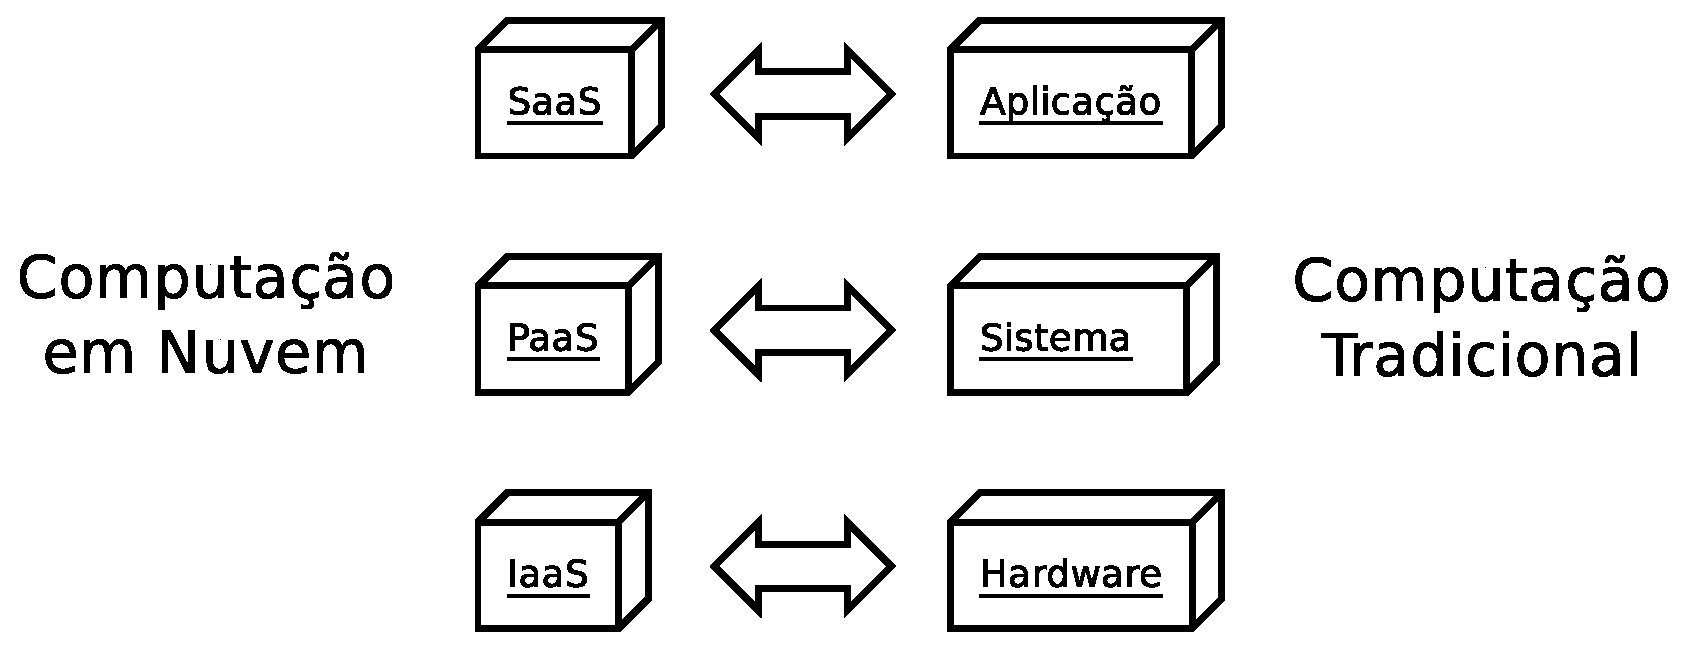
\includegraphics[width=0.99\textwidth]{img/arq-trad-nuvem.eps}
        \end{figure}
    
    \end{frame}
    
    \begin{frame}{Fundamentação Teórica}
    
        A Plataforma como um Serviço (\emph{Platform as a Services}) providencia um ambiente onde os desenvolvedores possam:

        \medskip
        \begin{itemize}
            \item Usar serviços e ferramentas para o desenvolvimento;
            \medskip
            \item Implantar aplicações;
            \medskip
            \item Gerenciar aplicações.
        \end{itemize}
    
    \end{frame}
    
    \begin{frame}{Fundamentação Teórica}
    
        Dependabilidade diz respeito a capacidade de entrega de um serviço que pode ser considerando confiável. Entre os principais atributos de dependabilidade estão:
        
        \begin{itemize}
            \item \textbf{Disponibilidade}: A capacidade de um sistema estar de prontidão para prover um serviço corretamente;
            \item \textbf{Confiabilidade}: A probabilidade que um sistema irá prover um serviço de forma contínua até uma instante de tempo $t$; 
            \item \textbf{Segurança}: Ausência de consequências catastróficas que poderiam afetar o(s) usuário(s) e o ambiente;
            \item \textbf{Integridade}: Ausência de alterações impróprias no estado de um sistema;
            \item \textbf{Manutenibilidade}: A habilidade para sofrer reparos e modificações;
            \item \textbf{Confidencialidade}: Ausência de divulgação desautorizada de informação.
        \end{itemize}

    \end{frame}
    
    \begin{frame}{Fundamentação Teórica}
    
        Cálculo de disponibilidade:
        
        \begin{align*}
   			Disponibilidade = \frac{MTTF}{MTTF + MTTR}
   		\end{align*}
    
        Tempo de indisponibilidade em um ano:
        
        \begin{align*}
   			Downtime_{anual} = (1 - Disponibilidade) \times 8760h
   		\end{align*}
   		
   		Número de noves:
   		
   		\begin{align*}
   			Nof9s = - log_{10}(1 - Disponibilidade)
   		\end{align*}
        
    \end{frame}

    \begin{frame}{Fundamentação Teórica}
    
        A função de confiabilidade $R(t)$ representa a probabilidade de que um sistema será operado sem falha em um intervalo de tempo entre 0 e $t$:
        
        \begin{align*}
            R(t) = P(T > t), t \ge 0
        \end{align*}
        
        onde $T$ é uma variável aleatória que representa o tempo para ocorrência de defeitos.
    
    \end{frame}
    
    \begin{frame}{Fundamentação Teórica}
    
        Modelos Combinatórios:

        \begin{itemize}
            \item FT - Árvore de Falha;
            \item RBD - Diagrama de Bloco de Confiabilidade;
            \item RG - Grafos de Confiabilidade.
        \end{itemize}
		
		\medskip \medskip
        
        Modelos Baseados em Estado:

        \begin{itemize}
            \item CTMC - Cadeias de Markov de Tempo Contínuo;
            \item SMP - Processos semi-Markov;
            \item SPN - Redes de Petri Estocáticas;
            \item GSPN - Redes de Petri Estocásticas Generalizadas;
            \item MRGP - Processo Regenerativo de Markov.
        \end{itemize}

    \end{frame}
    
    \begin{frame}

        \frametitle{Fundamentação Teórica}

        \begin{columns}[c] 
    
            \column{.45\textwidth}
                \begin{figure}[t]
                    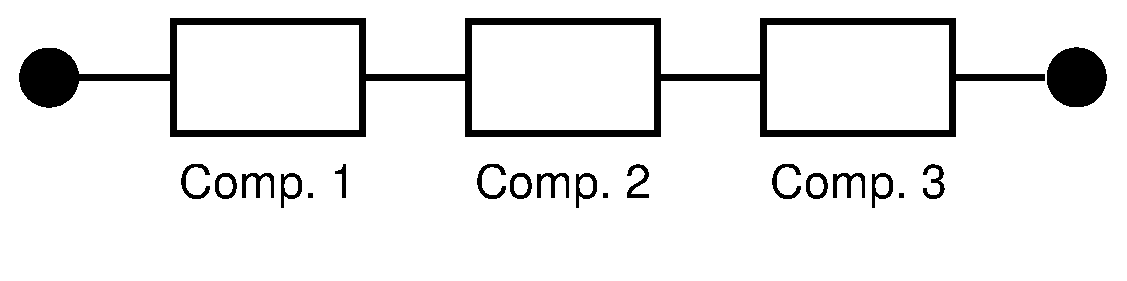
\includegraphics[width=0.96\textwidth]{img/EX_RBD_S.eps}
                \end{figure}
    
                \begin{align*}
                        R_{s} = \prod_{i = 1}^{n} R_i
                \end{align*}
    
            \column{.5\textwidth} 
        
                \begin{figure}[ht]
                    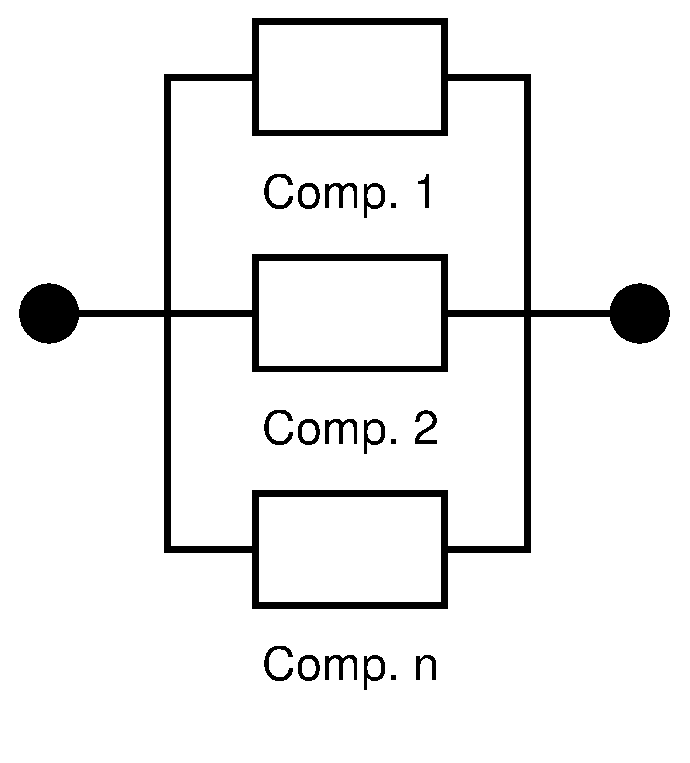
\includegraphics[width=0.56\textwidth]{img/EX_RBD_P.eps}
                \end{figure}
        
                \begin{align*}
                        R_{p} = 1 - \prod_{i = 1}^{n} (1 - R_i)
                \end{align*}
    
        \end{columns}

    \end{frame}

    \begin{frame}{Fundamentação Teórica}
    
        Cadeias de Markov é um \textbf{processo probabilístico} que apresenta a propriedade markoviana em que os \textbf{estados anteriores são irrelevantes para a predição dos estados seguintes}, para isso, o estado atual deve necessariamente ser conhecido. 
    
        \begin{figure}[ht]
            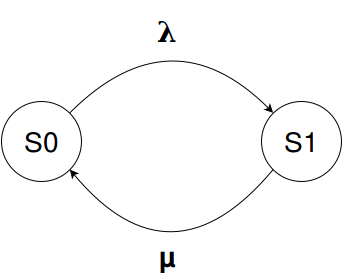
\includegraphics[width=0.3\textwidth]{img/ctmc_exemplo.png}
        \end{figure}
    
    \end{frame}
    
    \begin{frame}{Fundamentação Teórica}
    
        A análise de sensibilidade é uma técnica utilizada para \textbf{determinar os fatores} que possuem \textbf{maior relevância} sobre as medidas ou saídas de um modelo.
        
        Técnicas:
        
        \begin{itemize}
            \item Análise Diferencial;
            \item Análise de Correlação;
            \item Análise de Regressão;
            \item Análise de Perturbação;
            \item Design Experimental Fatorial.
        \end{itemize}
        
    \end{frame}
    
    \begin{frame}{Fundamentação Teórica}
    
        Termos importantes em DoE:

        \begin{itemize}
            \item Variável resposta;
            \item Fatores;
            \item Níveis.
        \end{itemize}
        
        Fatorial Completo:
        
        \begin{align*}
            num = \prod_{i = 1}^{k} (n_i)
        \end{align*}
        
        onde $k$ é o número de fatores, com o $i$-ésimo fator tendo $n_{i}$ níveis.
        
    \end{frame}
    
%----------------------------------------------------------------------------------------

\section{Metodologia}

    \begin{frame}{Metodologia}
        \Huge{\centerline{Metodologia}}
    \end{frame}

    \begin{frame}{Metodologia}

        \begin{figure}[ht]
            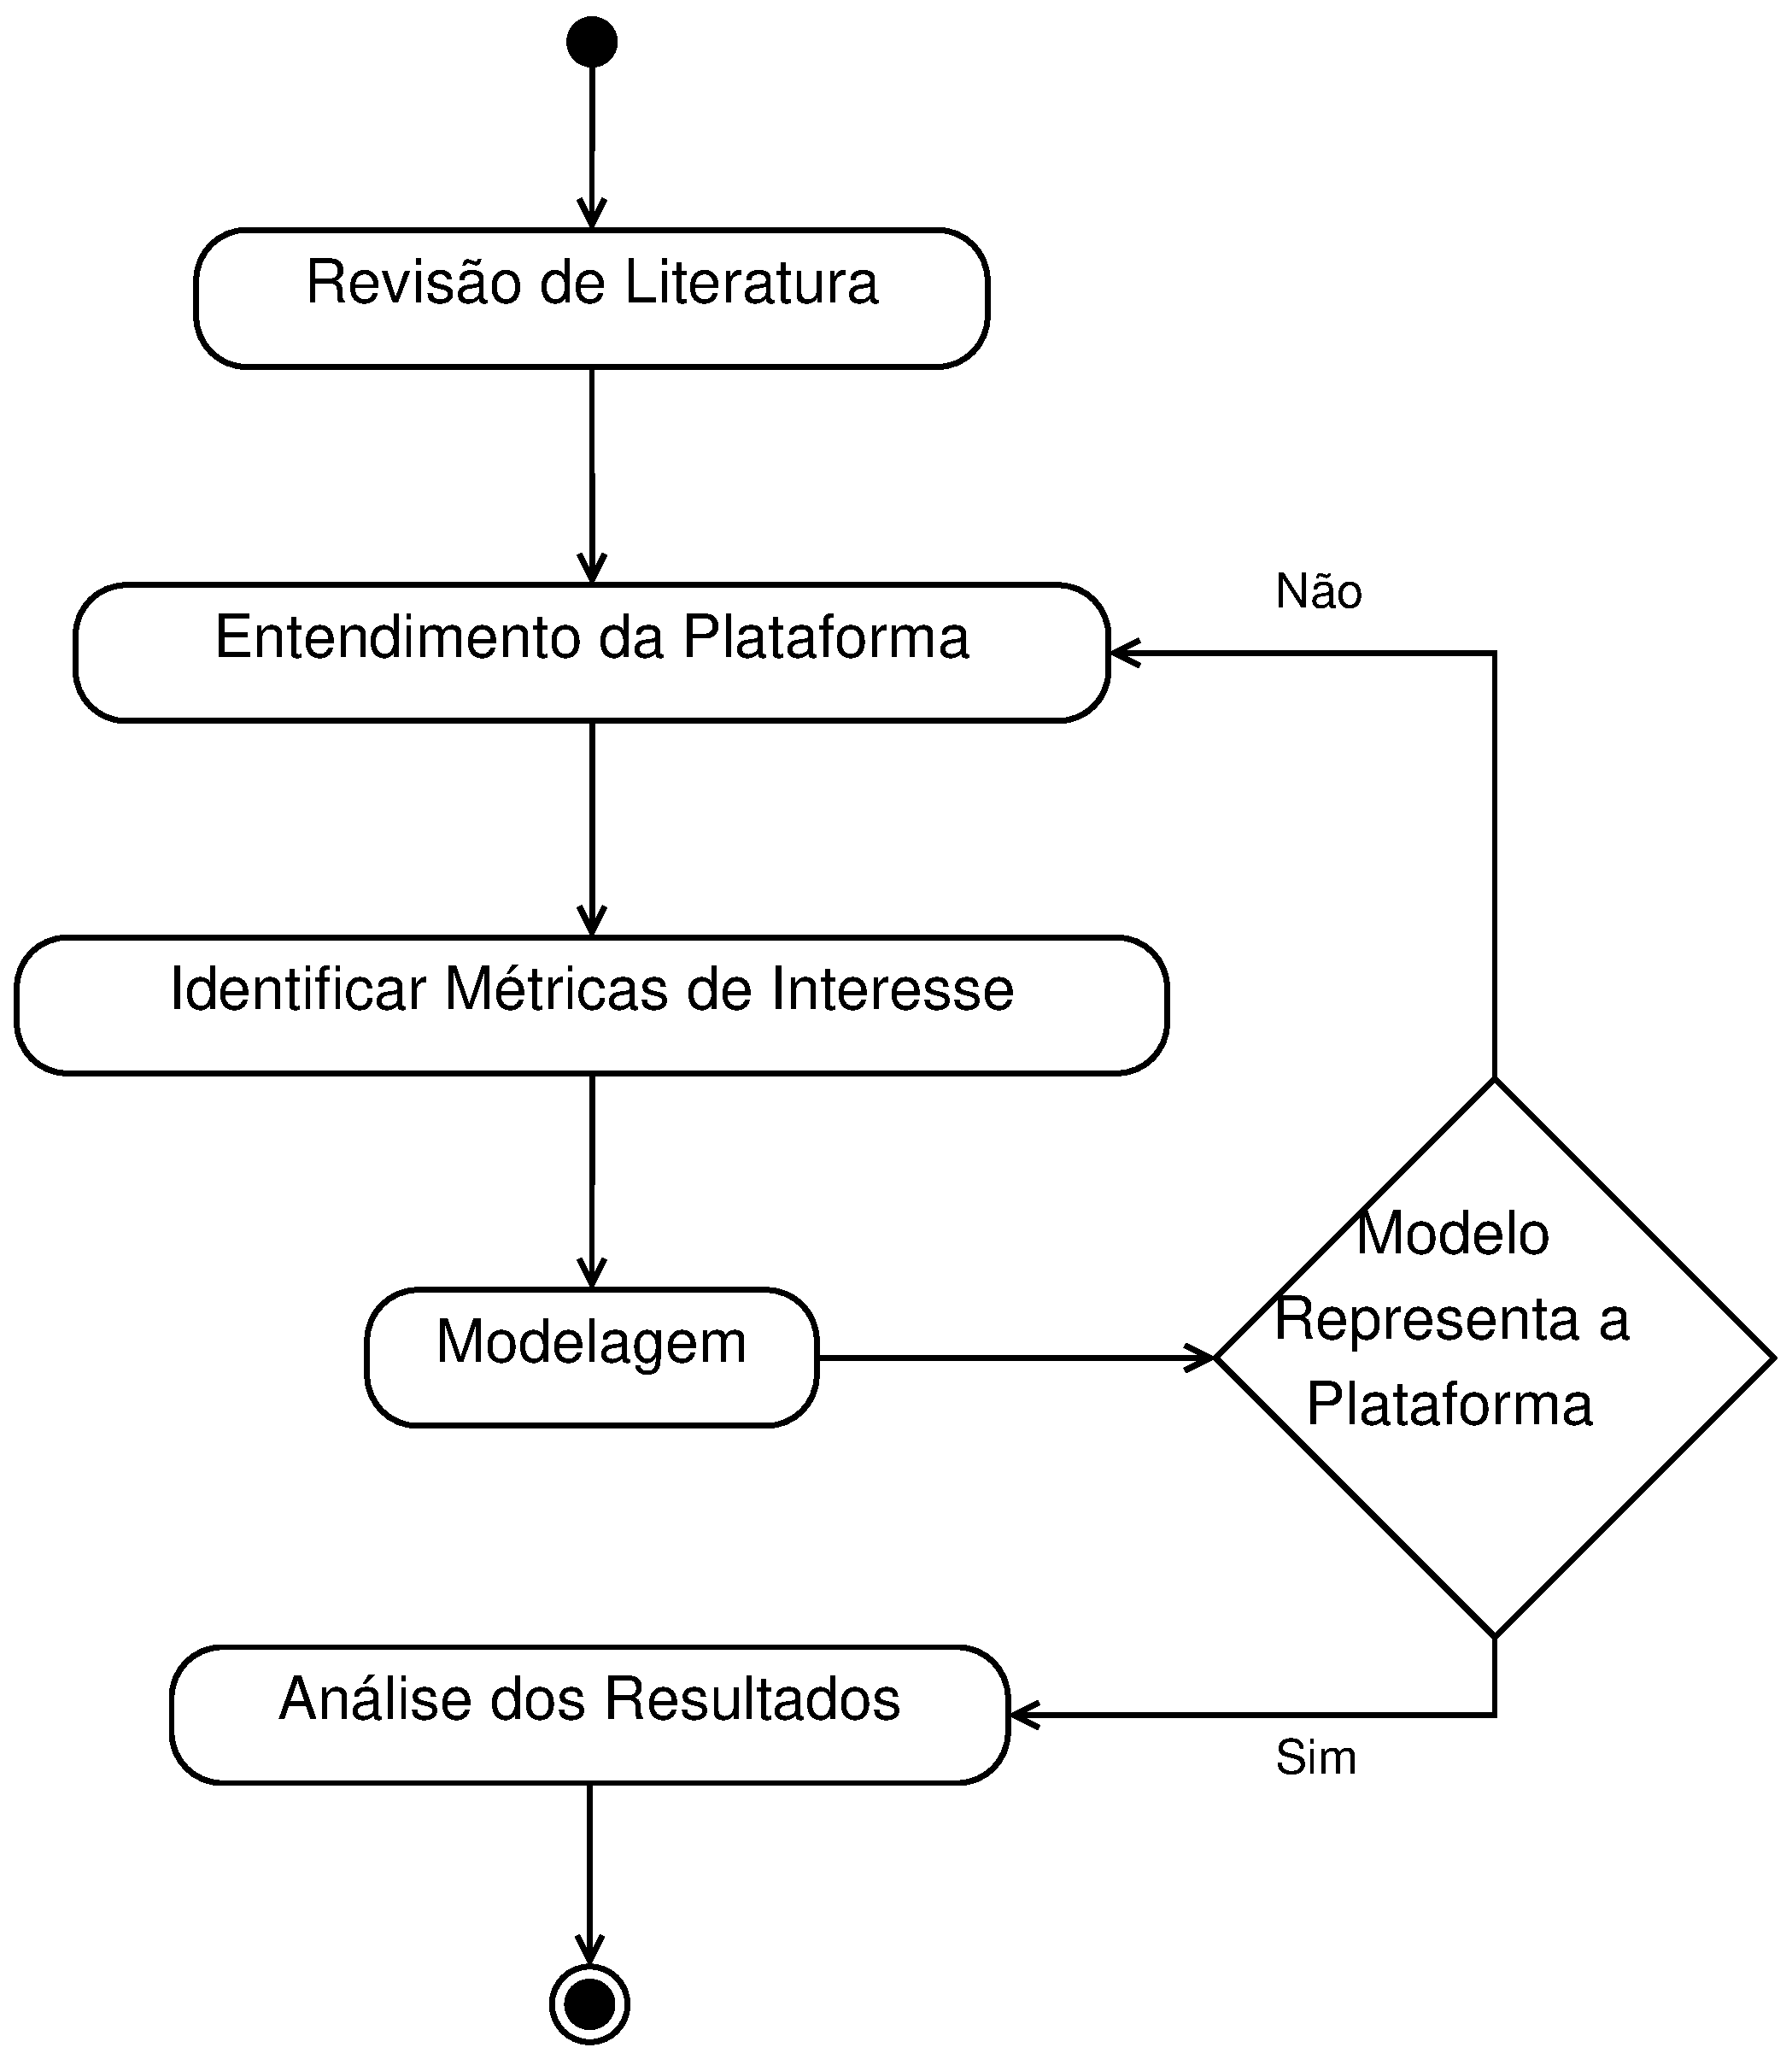
\includegraphics[width=0.50\textwidth]{img/metodos.eps}
        \end{figure}

    \end{frame}

    \begin{frame}{Metodologia}

        \begin{figure}[ht]
            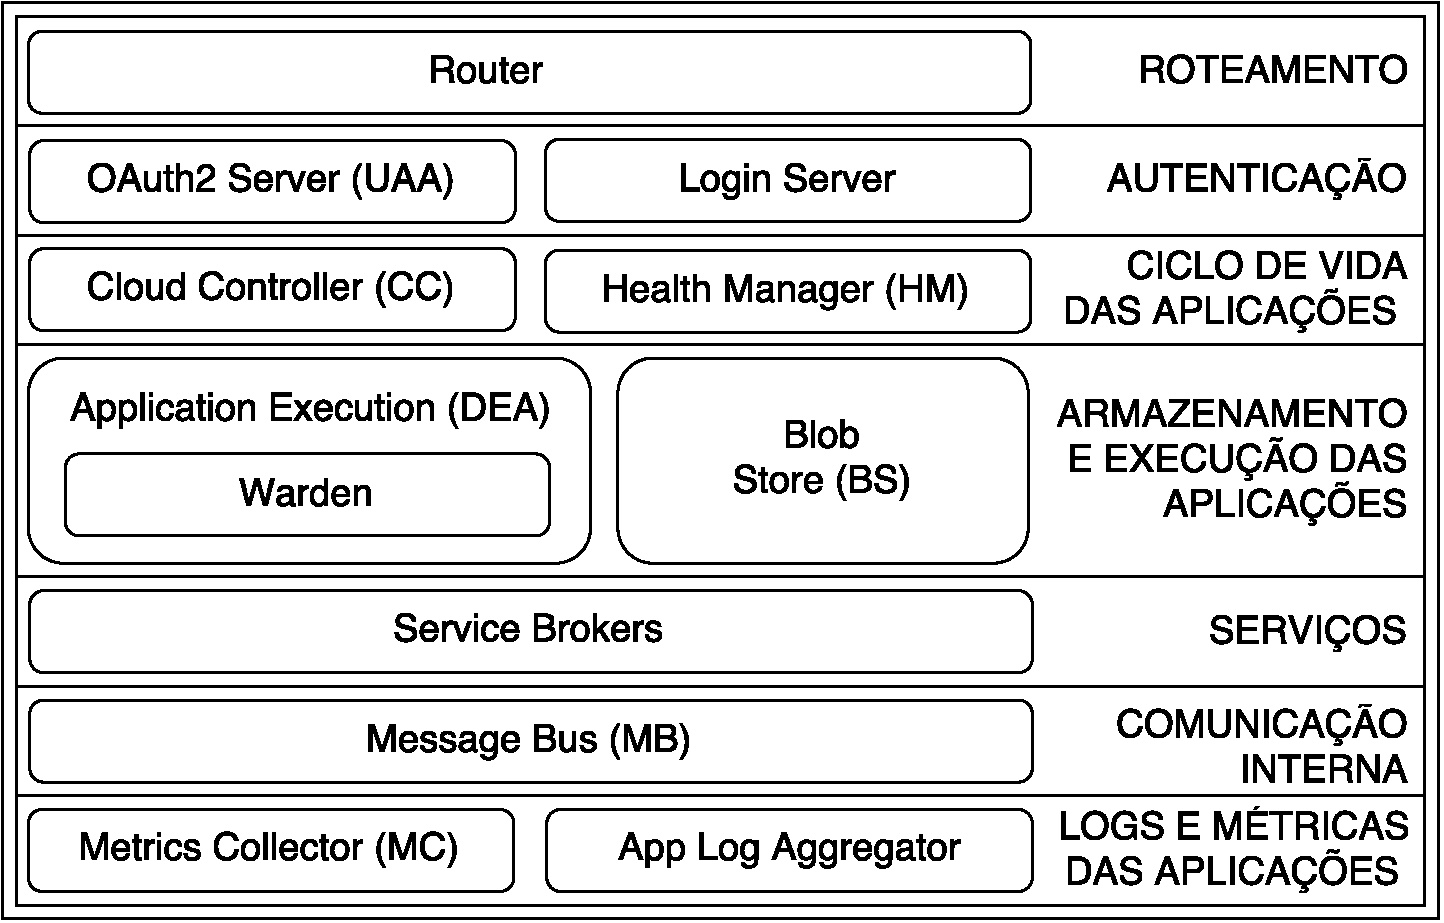
\includegraphics[width=0.80\textwidth]{img/arr_cf.pdf}
        \end{figure}

    \end{frame}    

    \begin{frame}{Metodologia}
    
        \begin{table}[h]
            \centering
            \begin{tabular}{@{}ll@{}}
            \toprule
            Componente        & Dependências        \\ \midrule
            Router            & --                 \\
            UAA               & JVM, Tomcat e SGBD \\
            CC                & Nginx, IR e SGBD   \\
            HM                & --                 \\
            DEA               & IR e Warden        \\
            Message Bus       & --                 \\
            Metrics Collector & IR                 \\ \bottomrule
            \end{tabular}
        \end{table}
    
    \end{frame}

%----------------------------------------------------------------------------------------

\section{Modelos Propostos}

    \begin{frame}{Modelos Propostos}
        \Huge{\centerline{Modelos Propostos}}
    \end{frame}
    
    \begin{frame}{Modelos Propostos}
    
        Modelo para o Cenário 1 (baseline)
        
        \begin{figure}[ht]
            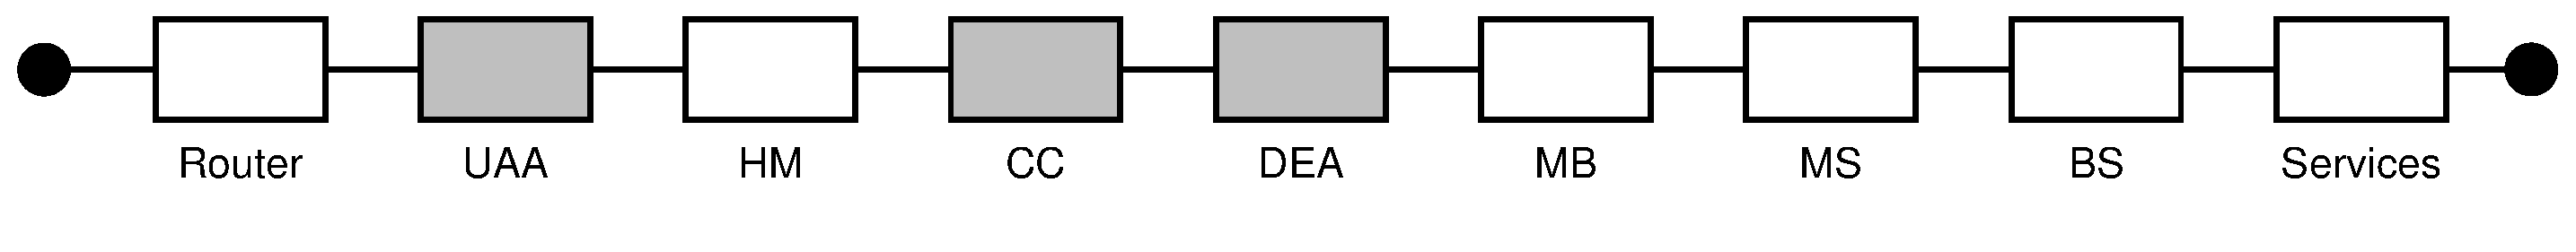
\includegraphics[width=0.9\textwidth]{img/model1}
        \end{figure}
        
        \begin{align*}
            D_{Cenario\_1} =~ & D_{Router} \times D_{UAA} \times D_{HM} \times D_{CC} \times\\
                            & D_{DEA}  \times  D_{MB} \times D_{MC} \times D_{BS}  \times D_{Services}
        \end{align*}

    \end{frame}
    
    \begin{frame}{Modelos Propostos}
    
        Modelo de Disponibilidade do UAA
    
        \begin{figure}[ht]
            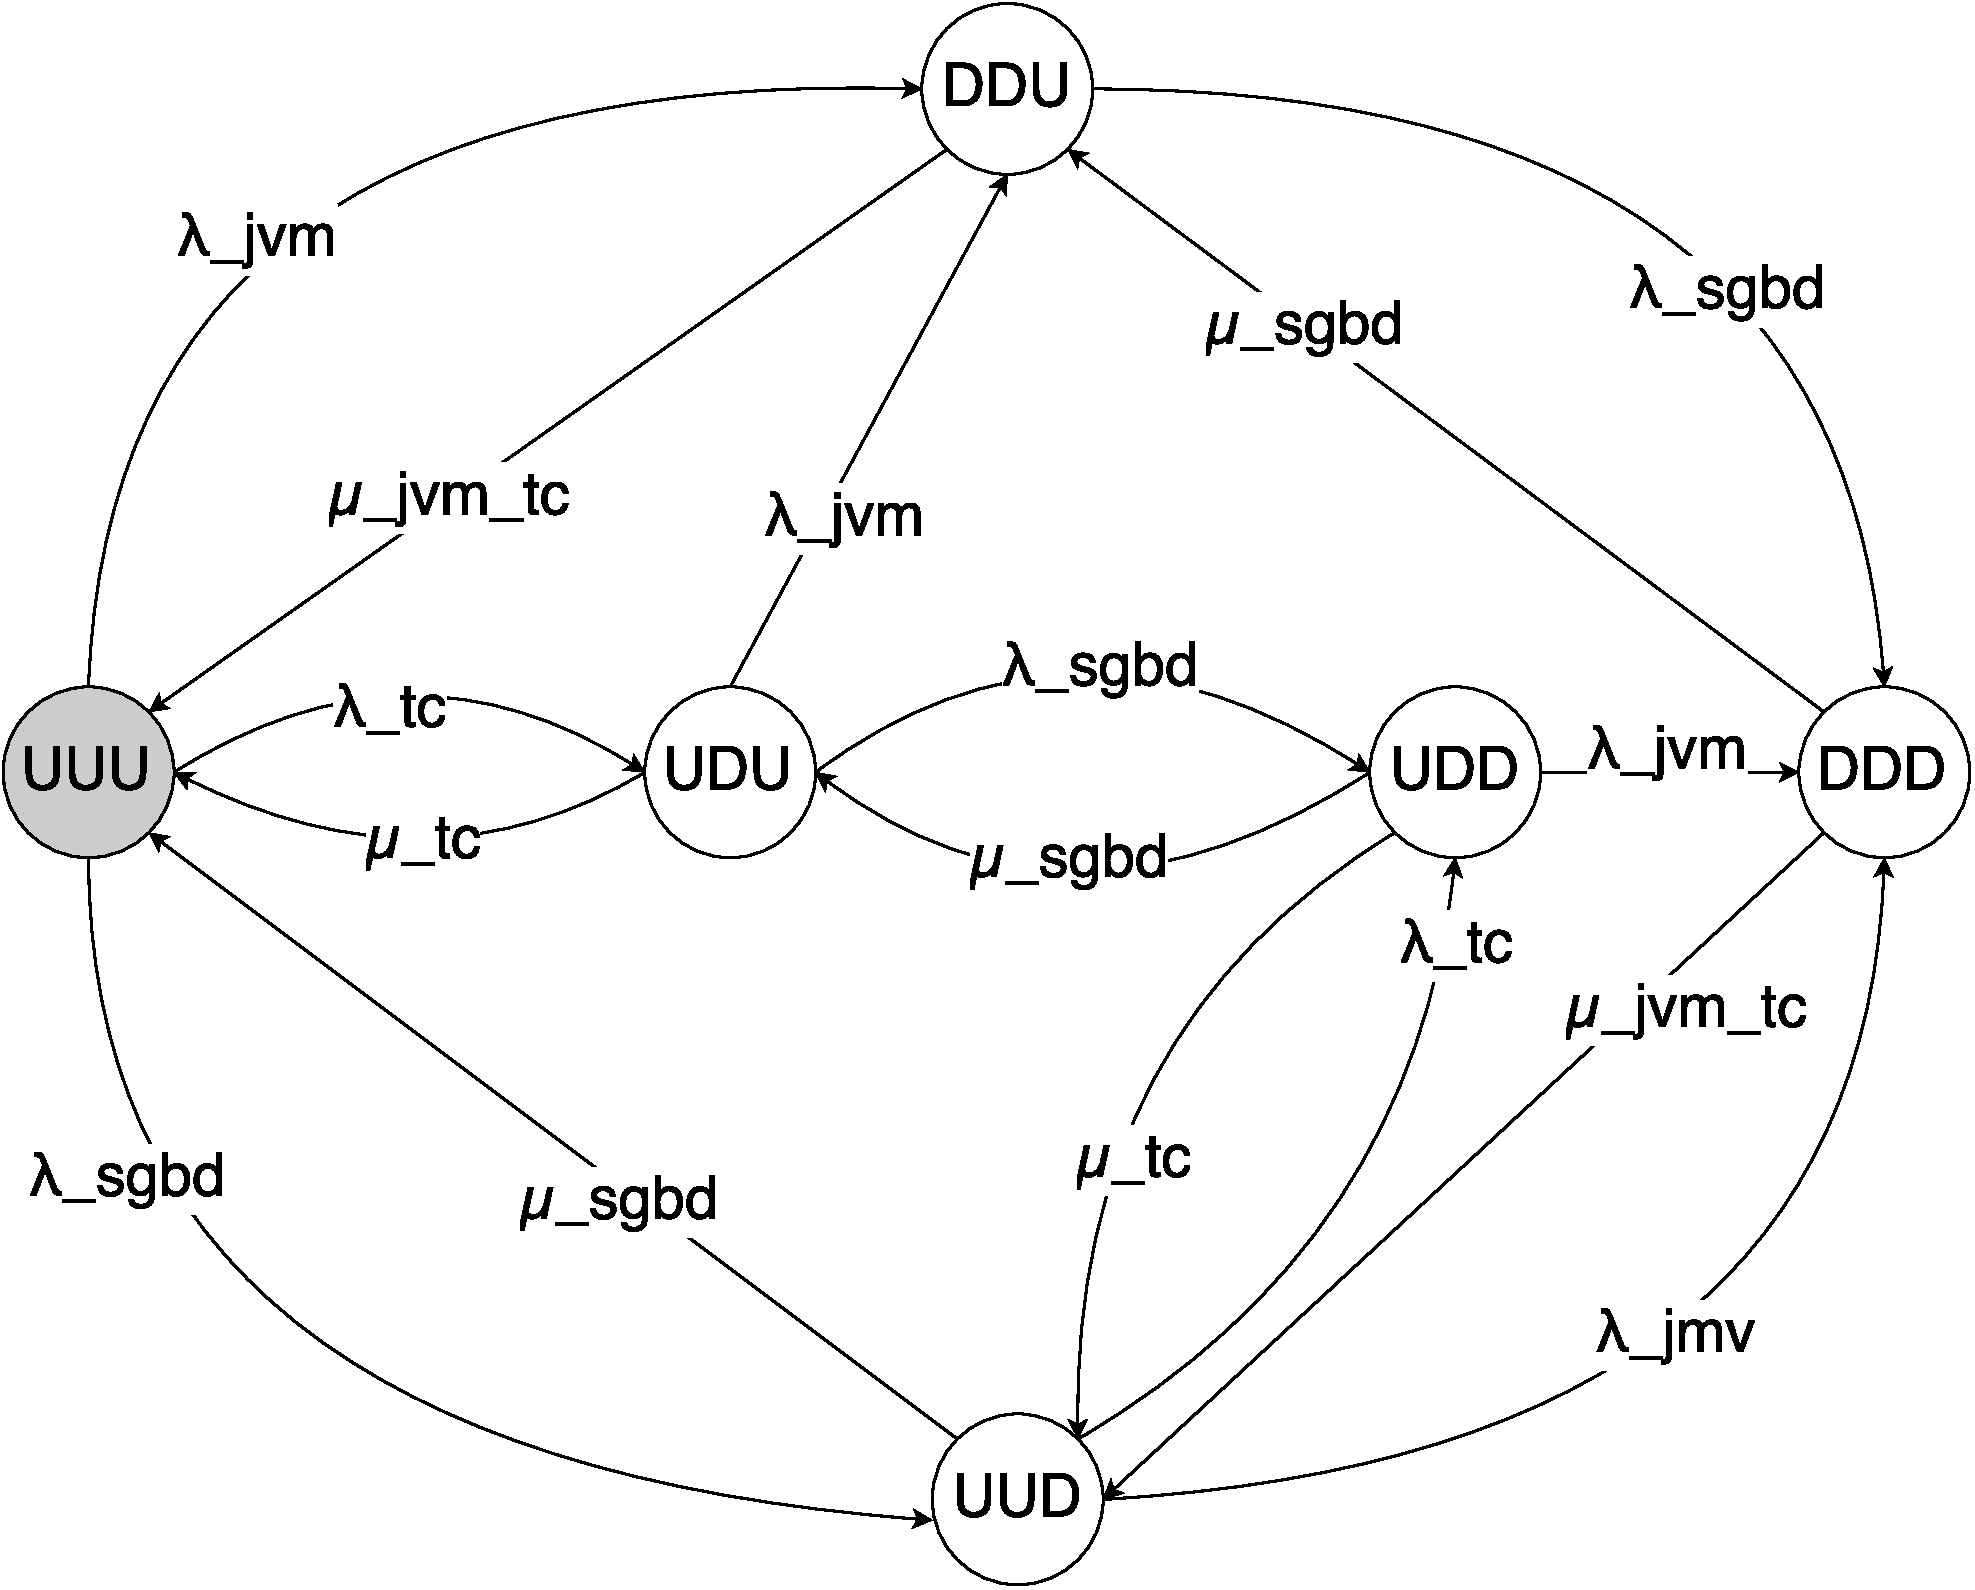
\includegraphics[width=0.50\textwidth]{img/cadeia-markov.pdf}
        \end{figure}
        
        \begin{align*}
         D_{UAA} = \frac{\mu_{SGBD} \times \mu_{JVM-TC} \times (\lambda_{JVM} \times \mu_{TC})}
                {(\lambda_{SGBD} + \mu_{SGBD}) \times (\lambda_{JVM} + \mu_{JVM-TC}) \times (\lambda_{JVM} + \lambda_{TC} + \mu_{TC})}
        \end{align*}

    \end{frame}
    
    \begin{frame}{Modelos Propostos}
        
        Modelo de Disponibilidade do CC
    
        \begin{figure}[ht]
            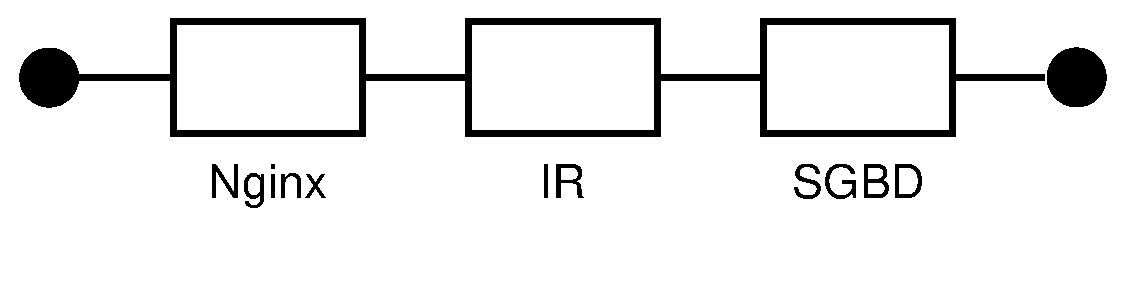
\includegraphics[width=0.4\textwidth]{img/cc.eps}
        \end{figure}
        
        \begin{align*}
            D_{CC} = D_{Nginx} \times D_{IR} \times D_{SGBD}
        \end{align*}

    \end{frame}
    
    \begin{frame}{Modelos Propostos}
    
        Modelo de Disponibilidade do DEA
        
        \begin{figure}[ht]
            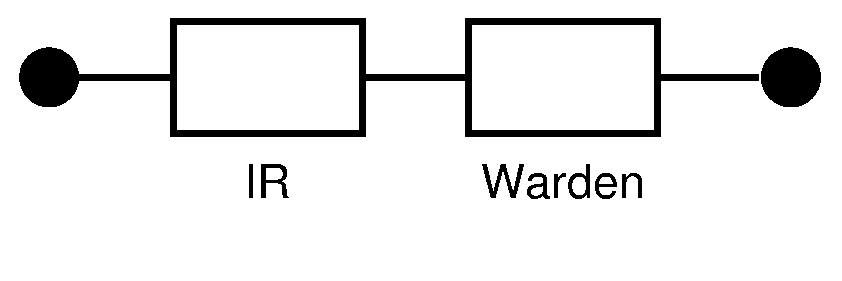
\includegraphics[width=0.3\textwidth]{img/dea.eps}
        \end{figure}
        
        \begin{align*}
            D_{DEA} = D_{IR} \times D_{Warden}
        \end{align*}

    \end{frame}
    
    \begin{frame}{Modelos Propostos}
    
        Modelo para o Cenário 2
        
        \begin{figure}[ht]
            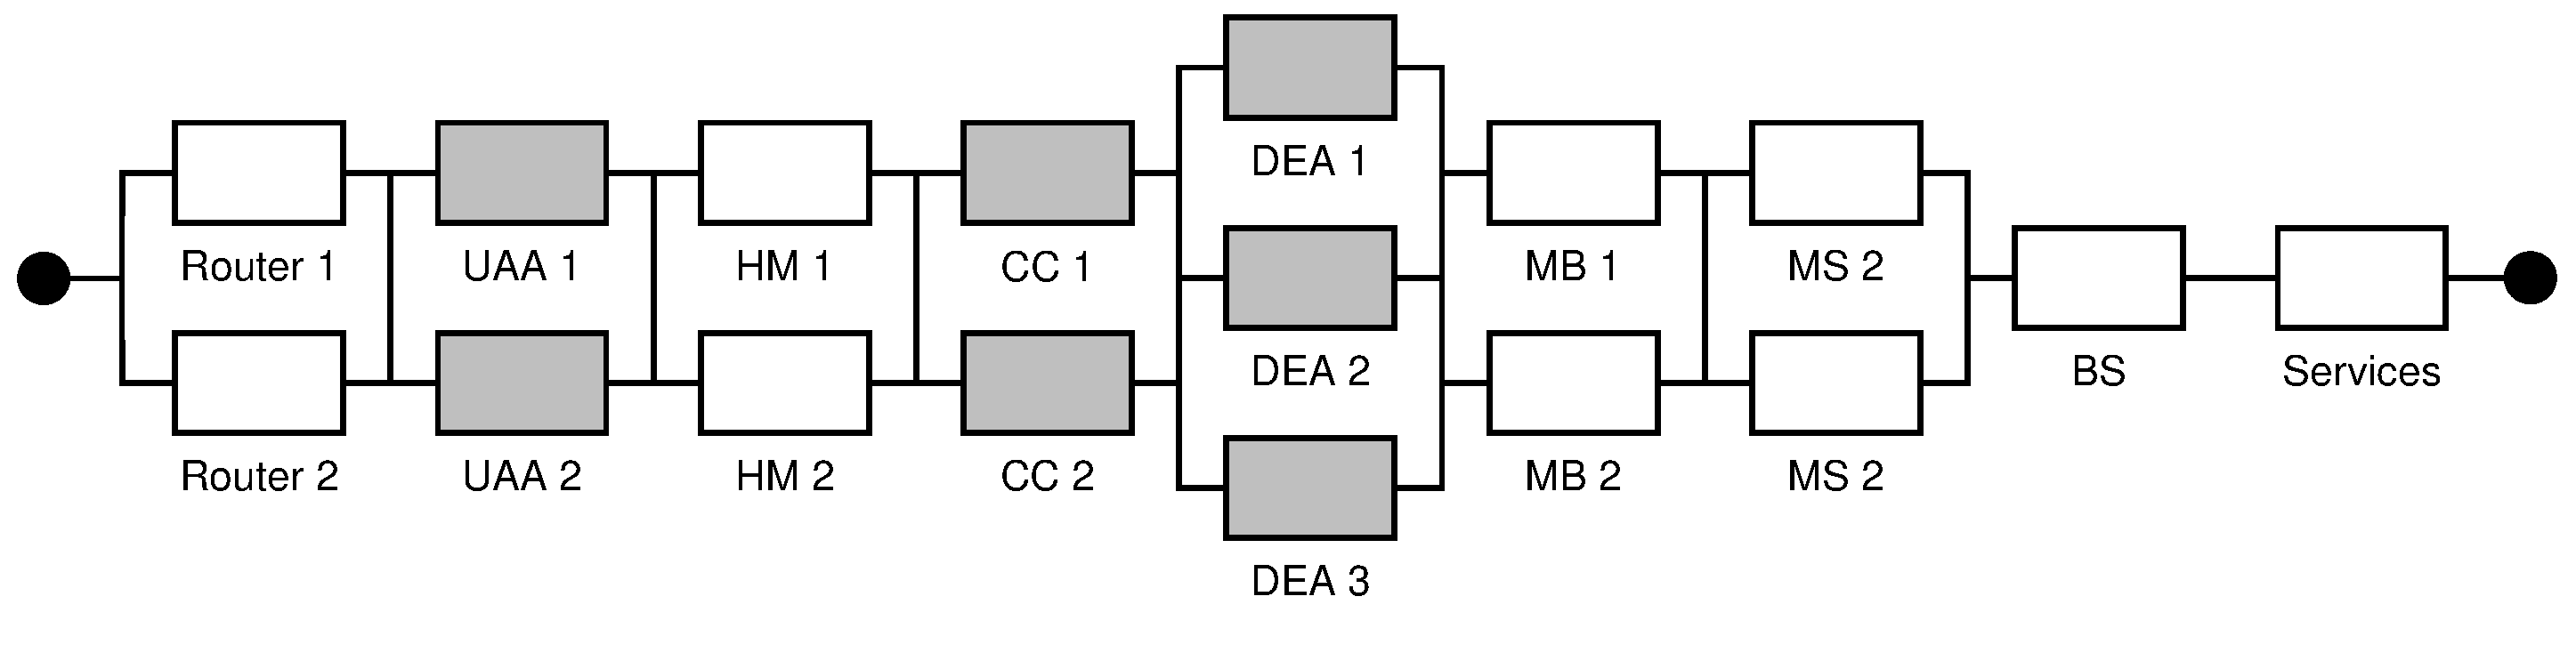
\includegraphics[width=0.9\textwidth]{img/model2}
        \end{figure}
        
        \begin{align*}
           D_{Cenario\_2}=~ & (1 - (1 - D_{Router})^2) \times (1 - (1 - D_{UAA})^2) \times \\
                            & (1 - (1 - D_{HM})^2) \times (1 - (1 - D_{CC})^2) \times (1 - (1 - D_{DEA})^3) \times  \\
                            & (1 - (1 - D_{MB})^2) \times (1 - (1 - D_{MC})^2) \times D_{BS} \times D_{Services}
        \end{align*}

    \end{frame}

    \begin{frame}{Modelos Propostos}
    
        Modelo para o Cenário 3
        
        \begin{figure}[ht]
            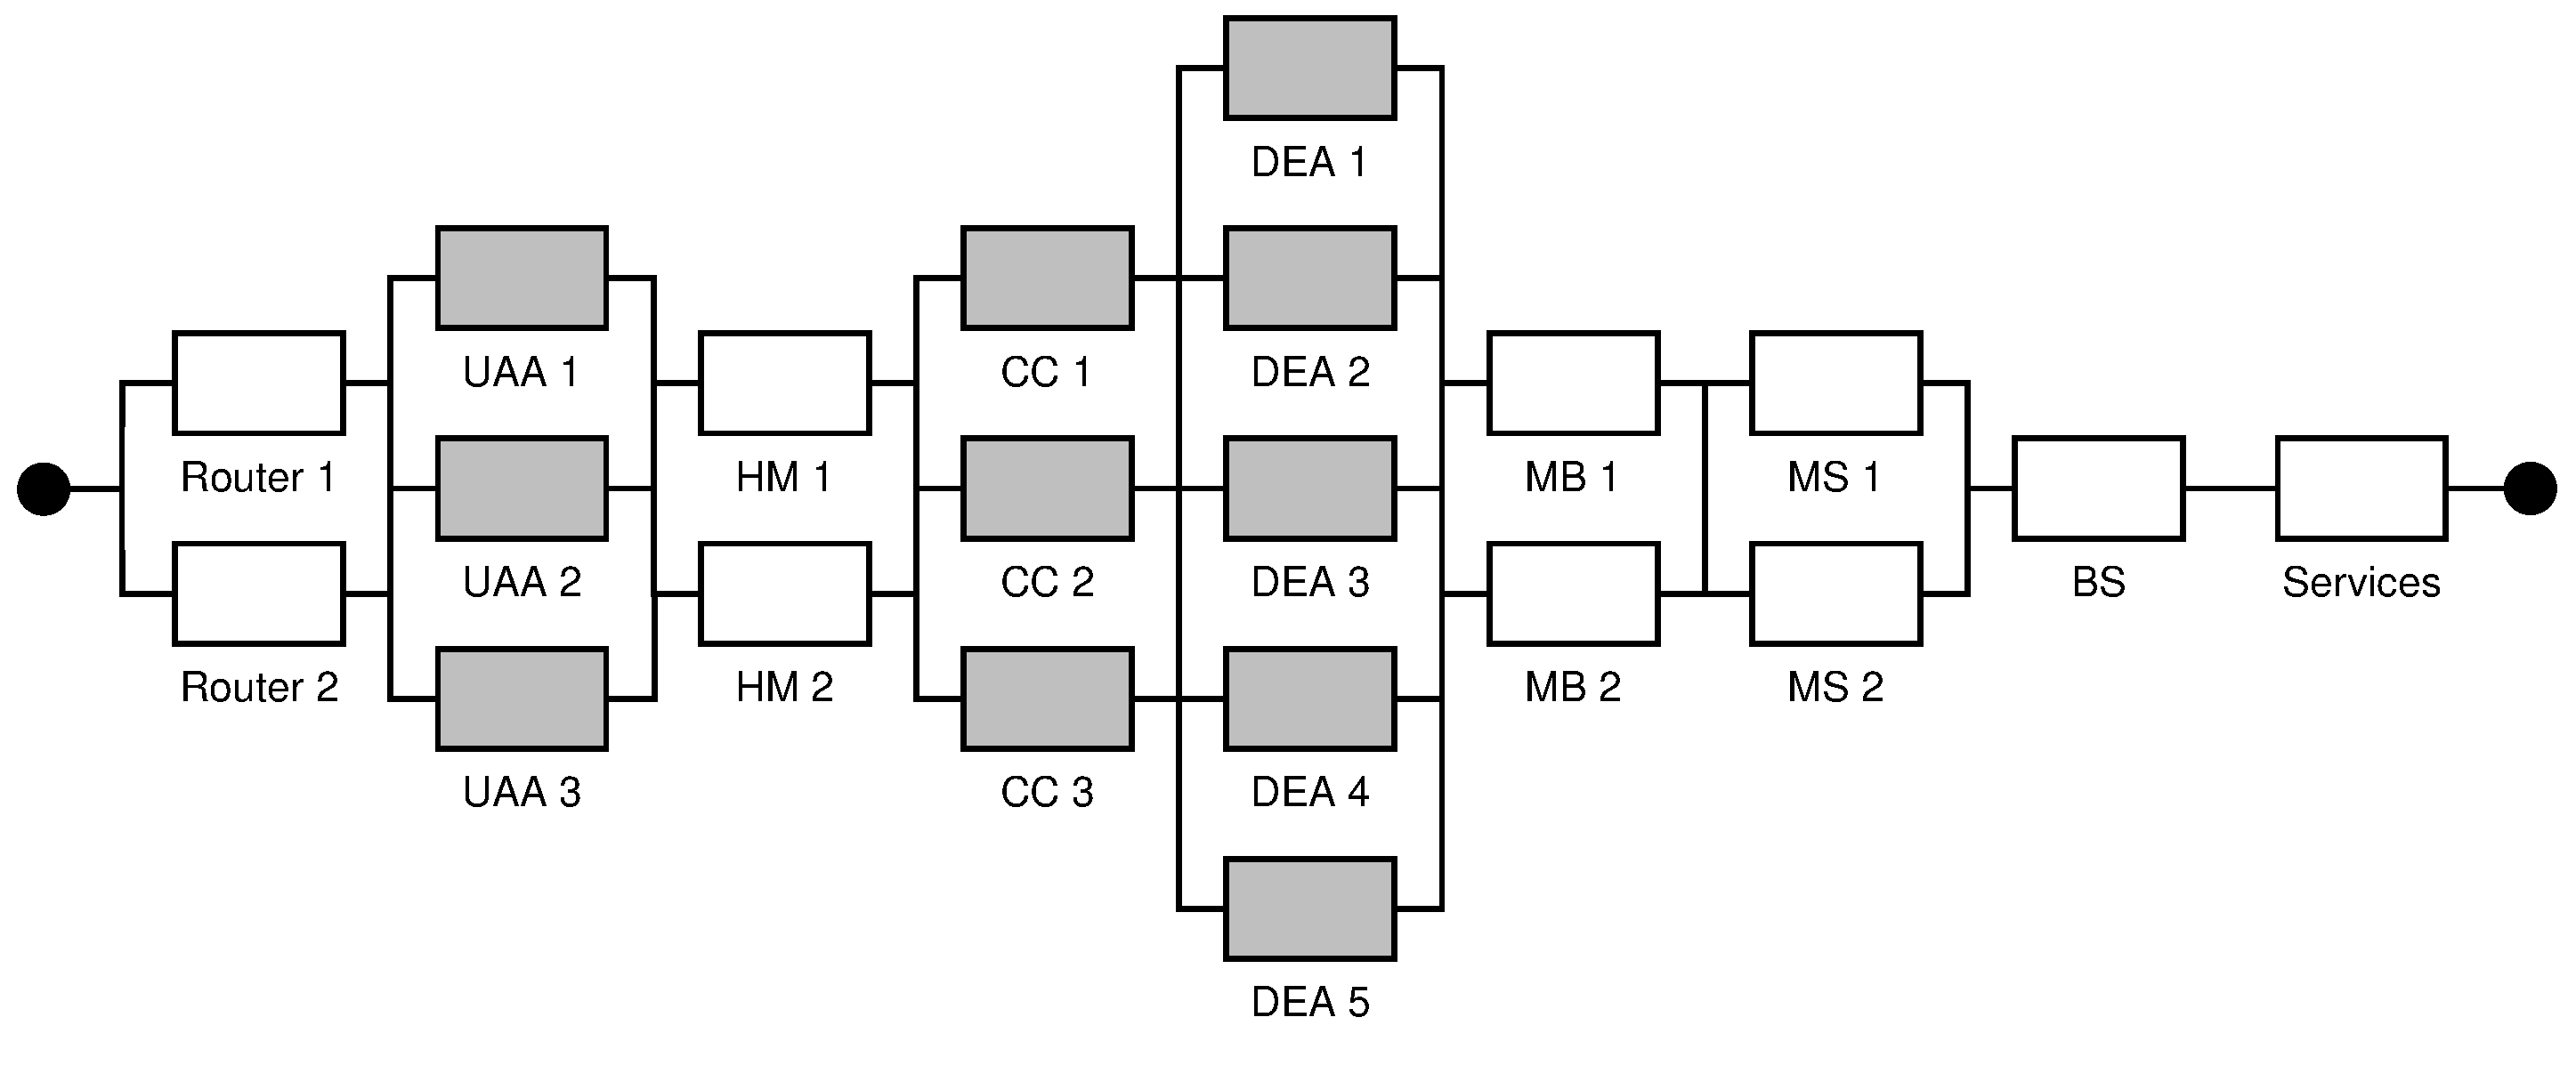
\includegraphics[width=0.9\textwidth]{img/model3}
        \end{figure}
        
        \begin{align*}
          D_{Cenario\_3} =~ & (1 - (1 - D_{Router})^2) \times (1 - (1 - D_{UAA})^3) \times \\
                            & (1 - (1 - D_{HM})^2) \times (1 - (1 - D_{CC})^3) \times (1 - (1 - D_{DEA})^5) \times \\
                            & (1 - (1 - D_{MB})^2) \times (1 - (1 - D_{MC})^2) \times D_{BS} \times D_{Services}
        \end{align*}

    \end{frame}

%----------------------------------------------------------------------------------------

\section{Resultados}

    \begin{frame}{Resultados}
        \Huge{\centerline{Resultados}}
    \end{frame}

    \begin{frame}{Resultados}
    
        Disponibilidade dos Componentes de Cloud Foundry
        
        \begin{table}[h]
        \centering
        \begin{tabular}{lr}
        \hline
        Componente        & Disponibilidade (\%) \\ \hline
        Router            & 99,87332            \\
        UAA               & 99,67830            \\
        HM                & 99,87332            \\
        CC                & 99,67758            \\
        DEA               & 99,74680            \\
        Message Bus       & 99,87332            \\
        Metrics Collector & 99,87332            \\
        Blob Store        & 99,87332            \\
        Services          & 99,87332            \\ \hline
        \end{tabular}
        \end{table}

    \end{frame}
    
    \begin{frame}{Resultados}
    
        Confiabilidade dos Cenários
    
        \begin{figure}[ht]
            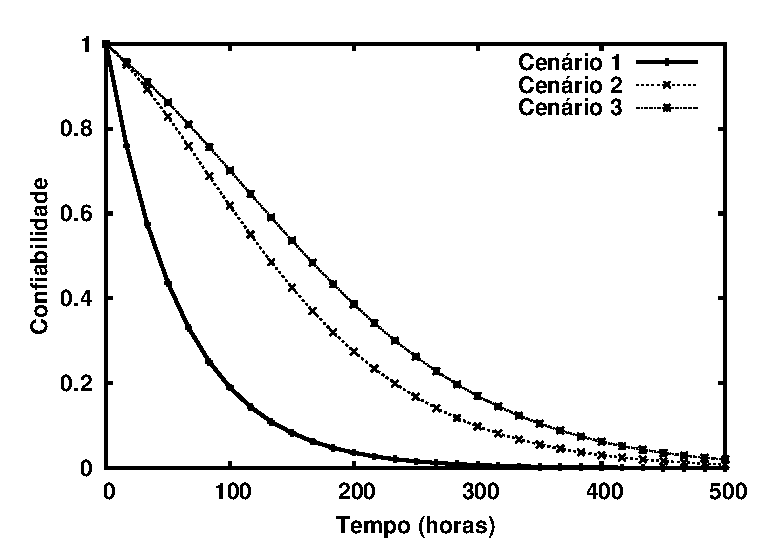
\includegraphics[width=0.70\textwidth]{img/confiabilidade.eps}
        \end{figure}
    
    \end{frame}
    
    \begin{frame}{Resultados}
    
        Disponibilidade dos Cenários
        
        \begin{table}[h]
        \centering
        \begin{tabular}{lrrr}
        \hline
        Métricas                    & \multicolumn{1}{l}{Cenário 1} & \multicolumn{1}{l}{Cenário 2} & \multicolumn{1}{l}{Cenário 3} \\ \hline
        Disponibilidade (\%)        & 98,35446                      & 99,74409                      & 99,74616                      \\
        Disponibilidade (N de 9's ) & 1,7836905                     & 2,5919169                     & 2,5954341                     \\
        \emph{Uptime} Anual (horas)        & 8615,7547                     & 8737,5676                     & 8737,7486                     \\
        \emph{Downtime} Anual (horas)      & 144,2553                      & 22,4324                       & 22,2514                       \\ \hline
            \end{tabular}
        \end{table}

    \end{frame}
    
    \begin{frame}{Resultados}
    
        Variação Paramétrica
        
        \begin{table}[h]
        \centering
        \begin{tabular}{lr}
        \hline
        Parâmetro       & \multicolumn{1}{l}{Valor (horas)} \\ \hline
        $MTTF_{Router}$ & 788,4                             \\
        $MTTR_{Router}$ & 1,0                               \\
        $MTTF_{DEA}$    & 393,944707812                     \\
        $MTTR_{DEA}$    & 1,0                               \\
        $MTTF_{UAA}$    & 309,848616791                     \\
        $MTTR_{UAA}$    & 1,0                               \\
        $MTTF_{CC}$     & 309,1544569                       \\
        $MTTR_{CC}$     & 1,0                               \\ \hline
        \end{tabular}
        \end{table}

    \end{frame}

    \begin{frame}{Resultados}

        \begin{figure}
            \centering
            {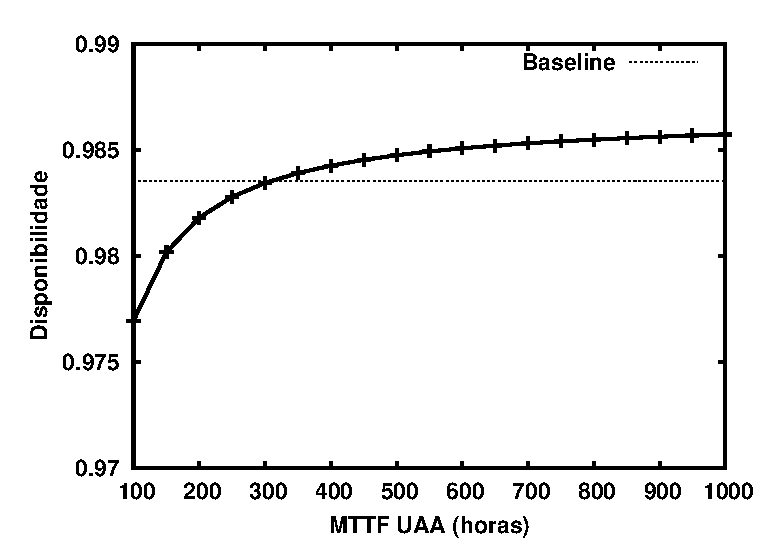
\includegraphics[width=0.42\textwidth]{img/mttf-uaa.eps}}\qquad
            {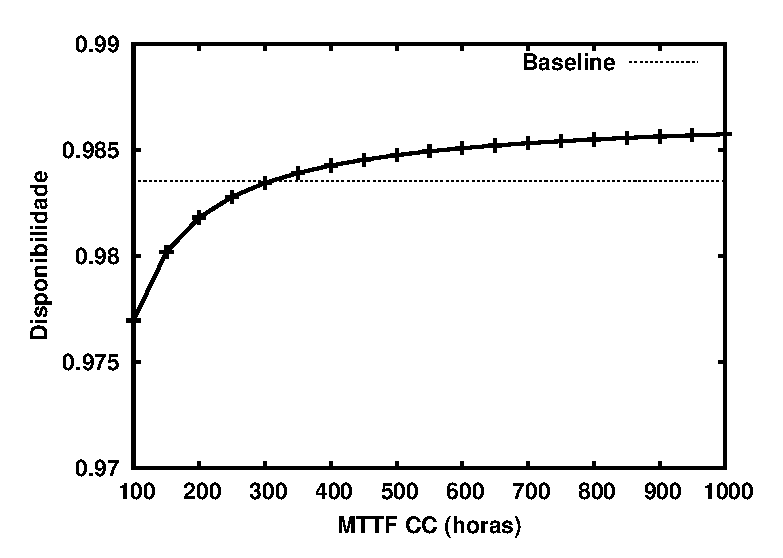
\includegraphics[width=0.42\textwidth]{img/mttf-cc.eps}}
        \end{figure}

        \begin{figure}
            \centering
            {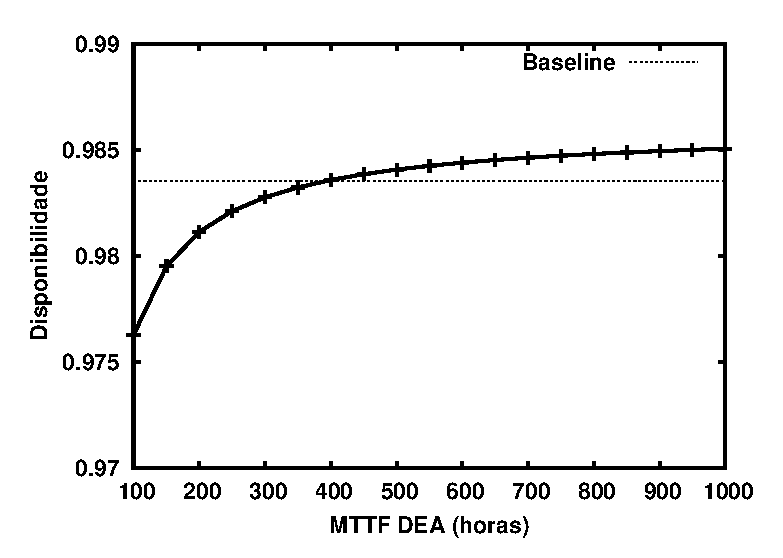
\includegraphics[width=0.42\textwidth]{img/mttf-dea.eps}}\qquad    
            {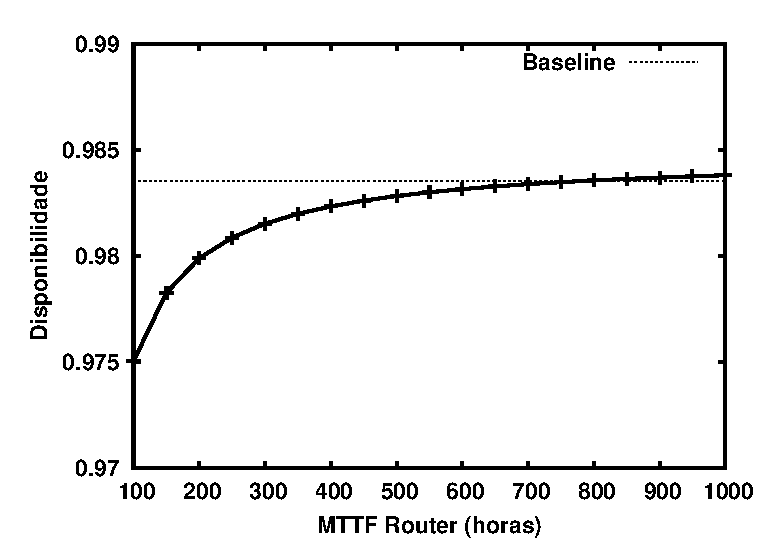
\includegraphics[width=0.42\textwidth]{img/mttf-router.eps}}
        \end{figure}

    \end{frame}    
    
    \begin{frame}{Resultados}

        \begin{figure}
            \centering
            {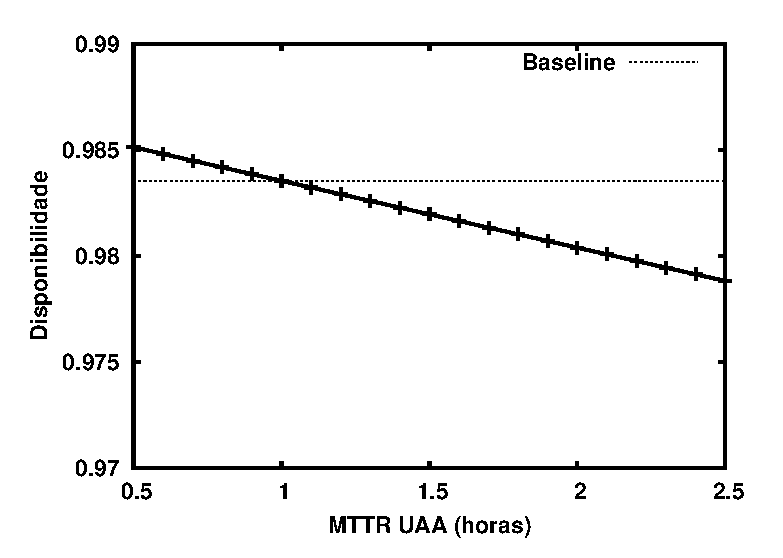
\includegraphics[width=0.42\textwidth]{img/mttr-uaa.eps}}\qquad
            {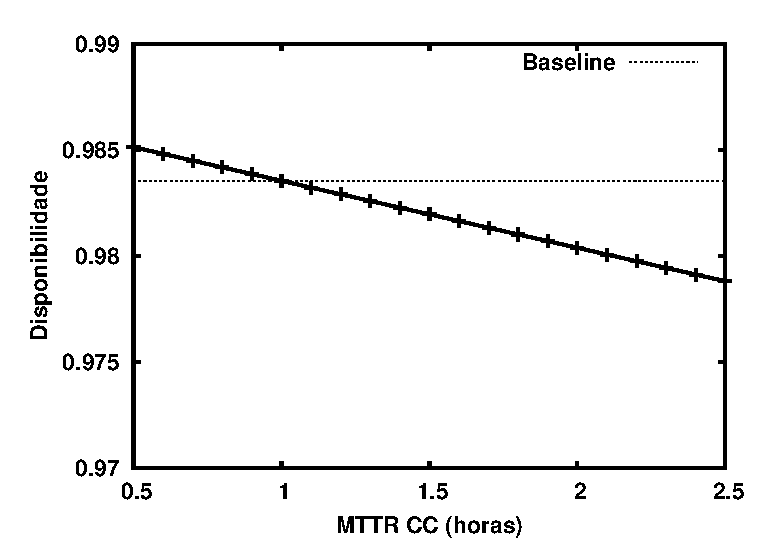
\includegraphics[width=0.42\textwidth]{img/mttr-cc.eps}}
        \end{figure}

        \begin{figure}
            \centering
            {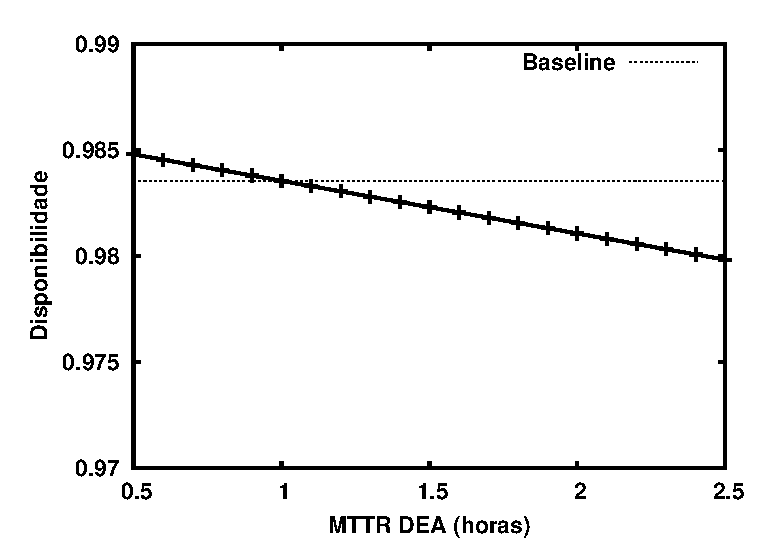
\includegraphics[width=0.42\textwidth]{img/mttr-dea.eps}}\qquad    
            {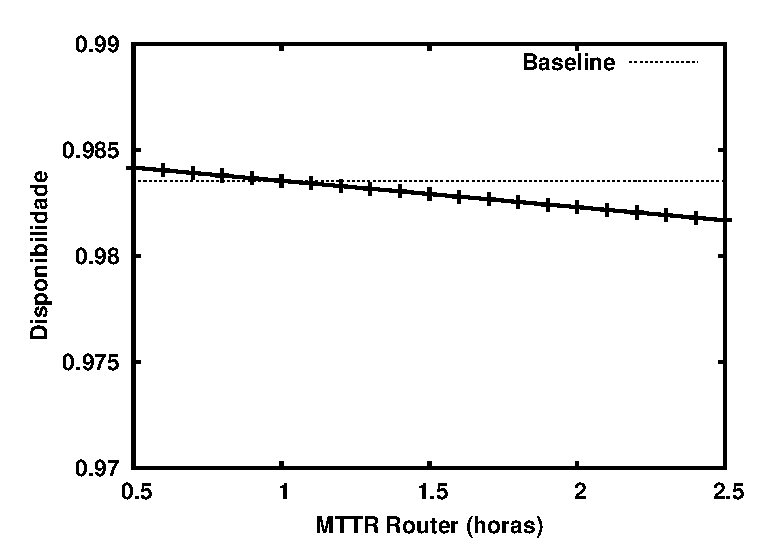
\includegraphics[width=0.42\textwidth]{img/mttr-router.eps}}
        \end{figure}

    \end{frame}
    


    \begin{frame}{Resultados}
    
        Análise de Sensibilidade DoE
        
        \begin{table}[h]
        \centering
        \begin{tabular}{lcr}
        \hline
        Fator  & Níveis & Valores       \\ \hline
        Router & 2      & 1, 2          \\
        UAA    & 3      & 1, 2, 3       \\
        HM     & 2      & 1, 2          \\
        CC     & 3      & 1, 2, 3       \\
        DEA    & 5      & 1, 2, 3, 4, 5 \\
        MB     & 2      & 1, 2          \\
        MC     & 2      & 1, 2          \\ \hline
        \end{tabular}
        \end{table}

    \end{frame}

    \begin{frame}{Resultados}

        \begin{figure}
            \centering
            \subfloat[Router]{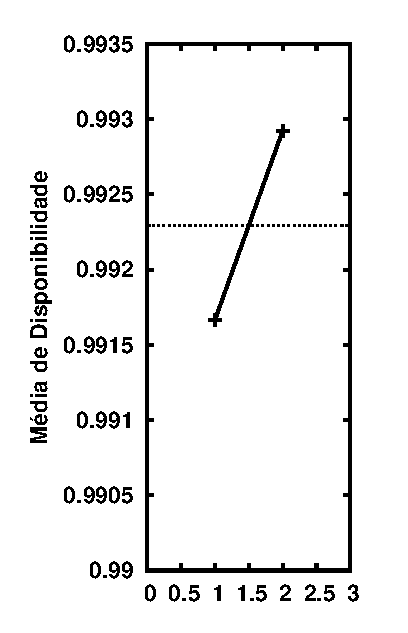
\includegraphics[width=0.149\textwidth]{img/doe-geral.eps}}
            \subfloat[UAA]{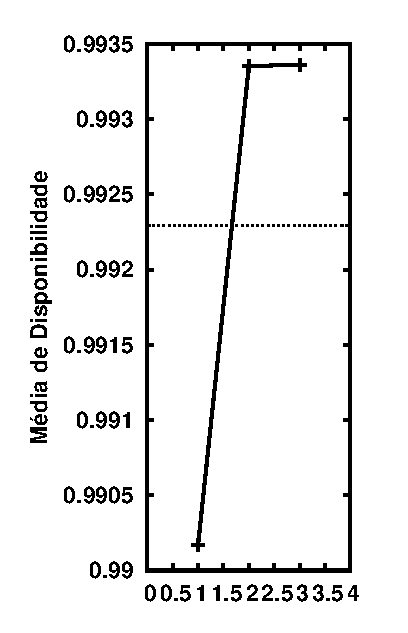
\includegraphics[width=0.149\textwidth]{img/doe-uaa.eps}}
            \subfloat[HM]{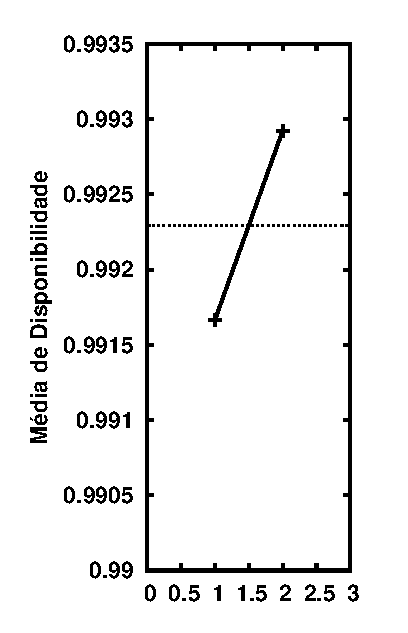
\includegraphics[width=0.149\textwidth]{img/doe-geral.eps}}
            \subfloat[CC]{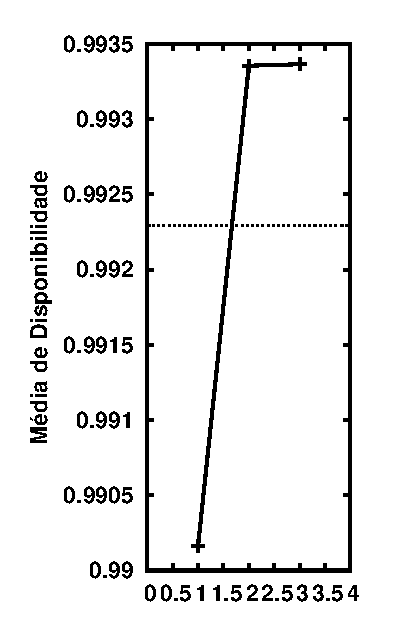
\includegraphics[width=0.149\textwidth]{img/doe-cc.eps}}
        \end{figure}

        \begin{figure}
            \centering
            \subfloat[DEA]{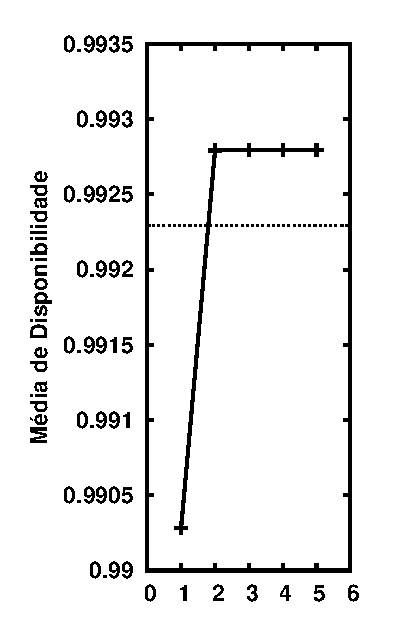
\includegraphics[width=0.149\textwidth]{img/doe-dea.eps}}
            \subfloat[MB]{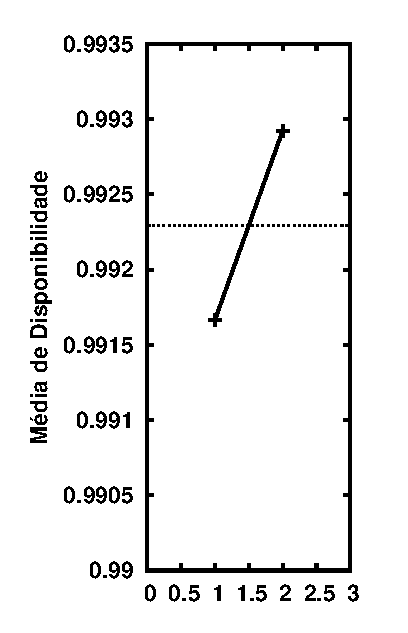
\includegraphics[width=0.149\textwidth]{img/doe-geral.eps}}
            \subfloat[MC]{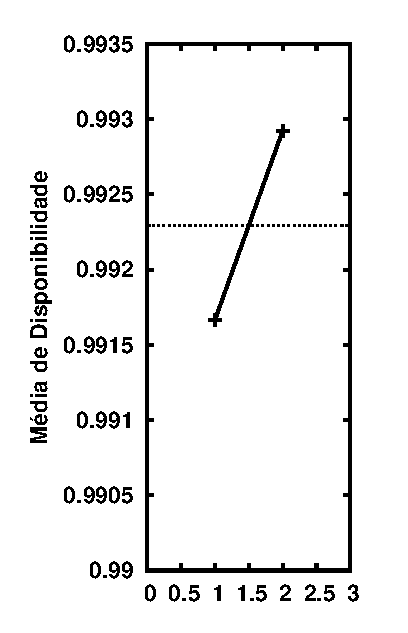
\includegraphics[width=0.149\textwidth]{img/doe-geral.eps}}
        \end{figure}

    \end{frame}
    
    \begin{frame}{Resultados}

        \begin{figure}[ht]
            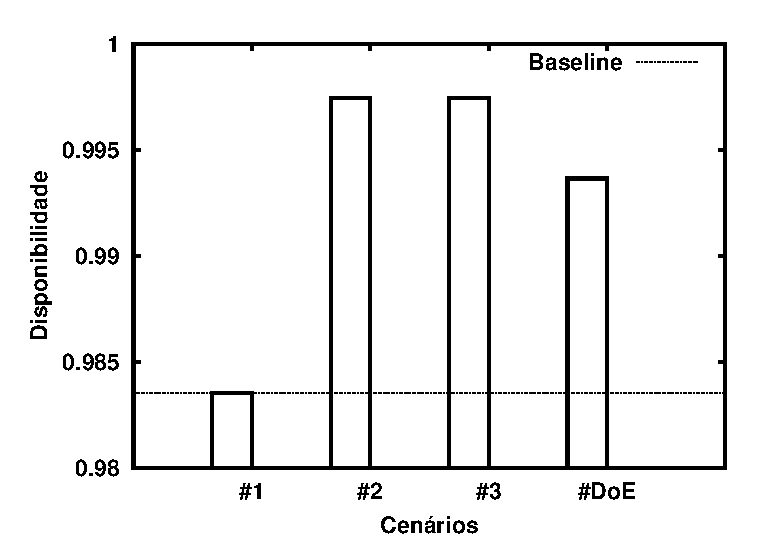
\includegraphics[width=0.70\textwidth]{img/disp-4-cenarios.eps}
        \end{figure}

    \end{frame}
      
    \begin{frame}{Resultados}

        \begin{table}[h]
        \centering
        \begin{tabular}{ccccr}
        \hline
        \multicolumn{1}{l}{Número de Nós Redundantes} & \multicolumn{1}{l}{UAA} & \multicolumn{1}{l}{CC} & \multicolumn{1}{l}{DEA} & \multicolumn{1}{l}{Disponibilidade (\%)} \\ \hline
        0                                             & 0                       & 0                      & 0                       & 98,35445                                \\
        1                                             & 0                       & 1                      & 0                       & 98,67156                                \\
        2                                             & 1                       & 1                      & 0                       & 98,98899                                \\
        3                                             & 1                       & 1                      & 1                       & 99,23963                                \\ \hline
        \end{tabular}
        \end{table}

    \end{frame}

%----------------------------------------------------------------------------------------

\section{Considerações Finais}

    \begin{frame}{Considerações Finais}
        \Huge{\centerline{Considerações Finais}}
    \end{frame}
    
    \begin{frame}{Considerações Finais}

        \begin{itemize}
        \item Os Cenários 2 e 3 tiveram resultados semelhantes nas análises de confiabilidade e disponibilidade;
        \item A variação paramétrica nos valores de MTTR influenciam de forma mais efetiva na disponibilidade dos componentes;
        \item Os componentes \emph{Services} e \emph{Blob Store} são os que mais prejudicam a disponibilidade da plataforma;
        \item Os componentes de maior sensibilidade a adição de nós redundantes são: DEA, UAA e CC.
        \item Uma implantação com mais de dois nós por componentes é pouco eficiente.
        \end{itemize}

    \end{frame}

    \begin{frame}{Considerações Finais}

        Trabalhos Futuros
        \begin{itemize}
        \item Estudos de caso com outras PaaS e considerando novos atributos de dependabilidade;
        \medskip
        \item Estudos considerando a IaaS.
        \end{itemize}

    \end{frame}
    
    \begin{frame}{}
        \Huge{\centerline{Obrigado!}}
    \end{frame}

\end{document} 